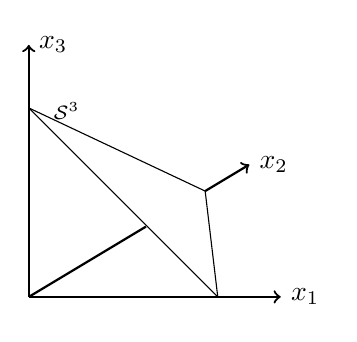
\begin{tikzpicture}[scale=0.8]

\draw [->,thick] (0,0) -- (0,4) node [right] {$x_3$};

\draw [->,thick] (0,0) -- (4,0) node [right] {$x_1$};

\draw [thick] (0,0) -- (1.86,1.116);

\draw [->,thick] (2.8,1.68) -- (3.5,2.1) node [right] {$x_2$};

\draw [] (0,3) -- (3,0);

\draw [] (0,3) -- (2.8,1.68);

\draw [] (3,0) -- (2.8,1.68);

\draw [] (0.6,2.95) node {\scriptsize $\mathcal{S}^3$};

% \draw [blue,dashed,semithick] (0,0) -- (1.5,1.5);
% %\draw [dotted,blue] (1.5,1.5) -- (1.88,1.88);
% \draw [blue,dashed,semithick] (1.88,1.88) -- (4,4);
% \draw [blue] (1.88,1.88) node {\tiny\textbullet};
% \node[minimum size=2pt,blue,fill,draw,circle,inner sep=0pt] () at (1.88,1.88){};
% \draw [blue] (1.91,1.68) node {\scriptsize $\mathcal{C}(\bm{w})$};

% \draw [blue] (3,3) node {\tiny\textbullet};
% \node[minimum size=2pt,blue,fill,draw,circle,inner sep=0pt] () at (3,3){};
% \draw [blue] (3.03,2.8) node {\scriptsize $\bm{w}$};

% \draw [blue,dashed,semithick] (0,0) -- (1.123,1.865);
% %\draw [dotted,blue] (1.123,1.865) -- (1.2,1.99);
% \draw [blue,dashed,semithick] (1.2,1.99) -- (2.83,4.7);
% %\draw [blue] (1.2,1.99) node {\tiny\textbullet};
% \node[minimum size=2pt,blue,fill,draw,circle,inner sep=0pt] () at (1.2,1.99){};


% \draw [blue,dashed,semithick] (2.8,0.49) -- (5.55,0.98);
% %\draw [dotted,blue] (2.55,0.45) -- (2.8,0.49);
% \draw [blue,dashed,semithick] (0,0) -- (2.55,0.45);
% \node[minimum size=2pt,blue,fill,draw,circle,inner sep=0pt] () at (2.8,0.49){};


\end{tikzpicture}

%%% Local Variables:
%%% mode: latex
%%% TeX-master: "../../../main"
%%% TeX-engine: xetex
%%% End:

